\documentclass[letterpaper,spanish]{article}
\usepackage{babel}
\usepackage[latin1]{inputenc}
\usepackage[pdftex]{graphicx}
\usepackage[dvipsnames,usenames]{color}
\usepackage{fancyhdr}
\usepackage{latexsym}
\usepackage{verbatim}

\oddsidemargin -0.3cm \topmargin -1.1cm \headheight 2.5cm
\textwidth 16.8cm \textheight 19.8cm

\newsavebox{\fondo}
\sbox{\fondo}{
\includegraphics[keepaspectratio,height=1.35\textheight,width=1.35\textwidth]{../../02_publicimage/margin.png}}

\pagestyle{fancy}
\fancyhead[C]{\setlength{\unitlength}{1in}
\begin{picture}(0,0)\put(-3.9,-9.3){\usebox{\fondo}}\end{picture}}

\renewcommand{\headrulewidth}{0pt}
\title{\huge{\textbf{DOCUMENTO DE AN�LISIS \\ Componentes de gesti�n de usuarios y autentificaci�n}}}
\author{Yeah! S.R.L.}
\date{\small{20 de marzo 2009}}

\begin{document}
\maketitle \pagebreak \tableofcontents \pagebreak

\section{INTRODUCCI�N}
Ante la necesidad de crear un sistema de gesti\'on de cursos y notas, para el apoyo a la evaluaci\'on de estudiantes,
se toma la decisi\'on de describir los recursos b\'asicos que poseer\'a el sistema.

En este documento se tratar\'a los asuntos relacionados al manejo de usuarios, sus categorias y la forma que
tienen estos de acceder al sistema.

\section{DESCRIPCI\'ON DEL PROBLEMA}

En todas las instituciones educativas se puede apreciar una forma de organizacion comun, como ser:
\begin{itemize}
    \item Profesor
    \item Ayudante
    \item Estudiantes
\end{itemize}
El Profesor y su(s) ayudante(s) trabajan juntos para coordinar el mejor modo de evaluar y dirigir su grupo, 
ya sea con trabajos practicos, cuestionarios, etc.; Por otra parte, los estudiantes tienen acceso a todos los 
documentos que han sido publicados por el profesor y el ayudante, y algo que es muy importante, los estudiantes 
pueden compartir informacion, es decir, publican archivos ya sea a todo el grupo o solo a su equipo.

\section{DESCRIPCI�N DE LA SOLUCI\'ON}

Como vimos en el punto 2, se tiene que pensar en tres actores principales: Profesor, Ayudante, y los Estudiantes.

Para cada usuario se tiene que pensar en las diferentes categorias que pueden tener como se muestra en la siguiente 
figura:

\begin{figure}[h]
    \centering
        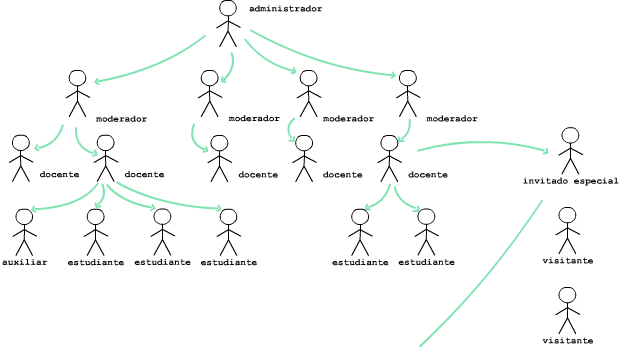
\includegraphics[width=0.6\textwidth]{images/module_categories.png}
    \caption{Categor\'ias de usuarios del sistema}
    \label{fig:categorias}
\end{figure}

\begin{description}
    \item[Administrador] Usuario encargado de la administraci�n del sistema.
    \item[Regente] Usuario encargado de la administraci�n de un espacio virtual.
    \item[Moderador] Usuario encargado de la administraci�n de una materia.
    \item[Docente] Usuario encargado de la administraci�n de un grupo.
    \item[Auxiliar] Usuario encargado de la colaboraci�n a un docente en su grupo.
    \item[Estudiante] Usuario registrado y que cursa un grupo de una materia.
    \item[Invitado] Usuario invitado por un Profesor, para el apoyo en intercambio de informaci\'on
    en su grupo o materia.
\end{description}

Cada una de estas categorias tiene diferentes funcionalidades, que dan lugar a la creaci\'on de roles para los usuarios:

\begin{figure}[h]
    \centering
        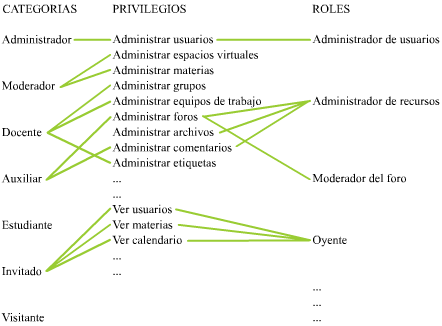
\includegraphics[width=0.7\textwidth]{images/module_roles.png}
    \caption{Categor\'ias del sistema y Roles}
    \label{fig:categorias}
\end{figure}

En la figura 1 se puede apreciar a un nuevo actor del sistema que es `Invitado', los Profesores pueden invitar a 
personas que consideren una ayuda importante en su grupo, podr\'a tener los mismos roles de un estudiante o m\'as, 
eso depende del Profesor de que clase de roles cree conveniente que tenga su invitado.

Ahora bien, hay dos formas que una persona ingrese como invitado a un grupo de una materia:
\begin{enumerate}
    \item Un profesor lo invite.
    \item Que una persona solicite ser parte de alg\'un grupo de esa materia, el ingreso de esa persona como 
    invitado del grupo depende de la autorizaci\'on del encargado(el Profesor del grupo).
\end{enumerate}

\begin{figure}[h]
    \centering
        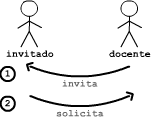
\includegraphics[width=0.2\textwidth]{images/module_invite.png}
    \caption{Formas de invitacion en el sistema}
    \label{fig:invitaciones}
\end{figure}

El usuario podr\'a ingresar al sistema mediante el ingreso de sus datos en un panel de acceso, tal como se muestra 
en la Figura 3. En el caso de que el usuario no pueda recordar su contrase\~na el sistema le enviar\'a una nueva 
contrase\~na a su correo electr\'onico.

\begin{figure}[h]
    \centering
        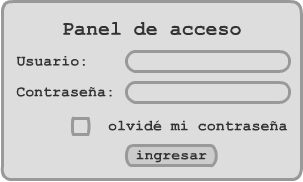
\includegraphics[width=0.4\textwidth]{images/module_login.png}
    \caption{Panel de acceso}
    \label{fig:invitaciones}
\end{figure}

\section{MODULOS PROPUESTOS}

\begin{description}
    \item [CATEGORY] Es el modulo de clasificaci\'on de los usuarios.
    \item [INVITE] Usuario invitado por un profesor, para el apoyo e intercambio de informaci\'on en el 
    grupo de una materia.
    \item [LOGIN] Es el que se encarga de permitir al usuario ingresar al sistema mediante su 
    nombre de usuario y contrase\~na.
    \item [ROLE] Brinda acceso/restricciones a funcionalidades/modulos del sistema.
    \item [USER] El modulo USER es el que se encarga de organizar a los diferentes tipos de usuarios
    del sistema mediante sus roles.
\end{description}

\section{FUNCIONES PROPUESTAS}
\subsection{CATEGORY}
    \begin {description}
        \item [Ver categorias] Permite ver la descripci\'on de la categor\'ia y los privilegios que tiene.
        \item [Editar categorias] Permite editar el t\'itulo y la descripci\'on de la categor\'ia.
        \item [Listar categorias] Lista todas las categorias con sus descripciones y privilegios.
        \item [Administrar categorias] Permite listar, editar y ver categorias.
    \end {description}
    
    \begin{figure}[h]
        \centering
            \includegraphics[width=0.6\textwidth]{images/usecase_category.png}
        \caption{Modulo CATEGORY}
        \label{fig:categorias}
    \end{figure}

\subsection{INVITE}
    \begin {description}
        \item [Solicitar acceso como invitado] Permite a un usuario ajeno al sistema solicitar invitacion a un grupo de una materia.
        \item [Ver solicitudes] El encargado de un grupo de la materia podr\'a ver todas las solicitudes para ingresar al sistema.
        \item [Denegar invitaci\'on] El encargado del grupo de la materia podr\'a denegar el acceso como invitado.
        \item [Brindar invitaci\'on] El encargado del grupo de la materia podr\'a brindar el acceso a la materia como invitado.
        \item [Listar invitaciones] Puede ver una lista de todos los invitados del grupo.
    \end {description}

    \begin{figure}[h]
        \centering
            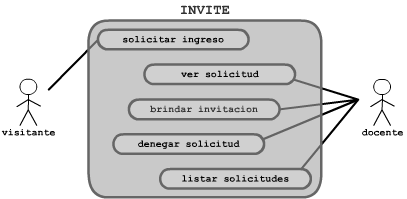
\includegraphics[width=0.6\textwidth]{images/usecase_invite.png}
        \caption{Modulo INVITE}
        \label{fig:categorias}
    \end{figure}

\subsection{LOGIN}
    \begin {description}
        \item [Ingresar al sistema] Permite validar y controlar el acceso del usuario.
        \item [Salir del sistema] Permite salir al usuario de una manera segura, terminando la sesi\'on de este.
        \item [Recuperar contrase\~na] El usuario env�a una solicitud de recuperar su contrase�a 
    \end {description}

    \begin{figure}[h]
        \centering
            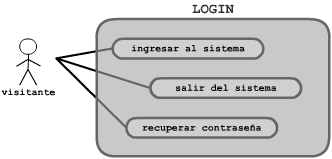
\includegraphics[width=0.6\textwidth]{images/usecase_login.png}
        \caption{Modulo LOGIN}
        \label{fig:categorias}
    \end{figure}

\subsection{ROLE}
    \begin {description}
        \item [Crear roles] Permite crear nuevos roles en base a las categor�as existentes. 
        \item [Editar Roles] Permite modificar el privilegio, descripci�n y t\'itulo del rol.
        \item [Asignar Roles] Permite asignar Roles a nuevos usuarios.
        \item [Ver roles] Permite ver la descripci�n y titulo que tiene un rol.
        \item [Administrar roles] Permite ver los privilegios que tiene un rol.
        \item [Eliminar roles] Permite eliminar una rol determinado.
        \item [Conceder privilegios] Permite conceder privilegios de una o mas categor�as, depende de los grados de libertad que se le quiere dar al rol.
        \item [Listar roles] Permite ver todos los roles existentes.
    \end {description}
    
    \begin{figure}[h]
        \centering
            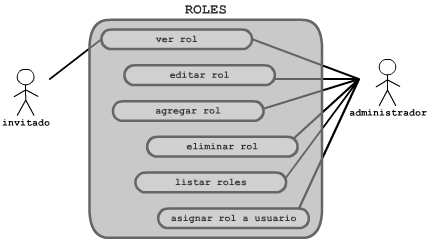
\includegraphics[width=0.6\textwidth]{images/usecase_roles.png}
        \caption{Modulo ROLE}
        \label{fig:categorias}
    \end{figure}

\subsection{USER}
    \begin {description}
        \item [Ver datos personales] Permite ver al usuario sus datos.
        \item [Editar datos personales] Permite al usuario editar sus datos.
        \item [Agregar usuario] Permite agregar nuevos usuario en el sistema.
        \item [Agregar un rol a un usuario] Permite agregar un rol determinado por el usuario que lo crea.
        \item [Bloquear un usuario] Permite bloquear su funcionalidad de un usuario, quiere decir que el usuario bloqueado no podr� hacer ninguna actividad en el sistema.
    \end {description}
    
    \begin{figure}[h]
        \centering
            \includegraphics[width=0.6\textwidth]{images/usecase_user.png}
        \caption{Modulo USER}
        \label{fig:categorias}
    \end{figure}

\section{RESTRICCIONES ENCONTRADAS}
Adicionalmente a las funcionalidades listadas se encontraron las siguientes alternativas de soluci\'on:
\begin{description}
    \item [Recordar contrase\~na] Permite al sistema guardar la session del usuario permanentemente.
    \item [Creaci\'on de formularios din\'amicos] Manipulacion dinamica de la informacion de los perfiles de usuario por parte de los docentes y administrador.
\end{description}

Dichas funcionalidades se han removido temporalmente para no afectar el tiempo estimado de desarrollo.

\begin{comment}
\vspace{0.5cm}

Le�do el presente documento, fu� revisado por un representante de la empresa TIS, juntamente con el representante de la grupo-empresa Yeah S.R.L., el director del proceso de analisis y sus colaboradores. Encontrandose las siguientes observaciones:

\vspace{5cm}
    \begin{table}[htbp]
        \begin{center}
            \begin{tabular}{c c}
\_\_\_\_\_\_\_\_\_\_\_\_\_\_\_\_\_\_\_\_\_\_\_\_\_\_\_\_\_\_\_\_\_\_\_\_\_\_\_\_\_\_\_ &
\_\_\_\_\_\_\_\_\_\_\_\_\_\_\_\_\_\_\_\_\_\_\_\_\_\_\_\_\_\_\_\_\_\_\_\_\_\_\_\_\_\_\_ \\
Lic. Leticia Blanco Coca & Luis Arce Claros \\
Representante legal de la empresa TIS & Director del proceso de analisis de la empresa Yeah! S.R.L.\\
            \end{tabular}
        \label{tab1}
        \end{center}
    \end{table}
\end{comment}

\end{document}
